\chapter{Introduction}

Human memory has been studied by psychologists and neurologists for about 100 years~\cite{baddeley1997human}, it is the biological storage for the information acquired from past experience with the environment. There are many types of memory, all cooperating in the process of memorization. It may seem that memory is a single unitary system such as the heart, however, it is rather a collection of systems where for example one system is responsible for the encoding of new information while another helps with its storage over a long period of time.

The systems responsible for retention of information in the human brain are very closely related to \textit{learning} and \textit{forgetting}, both of which additionally depend to some extent on memory. That is true because our memory provides the means and structure to link new knowledge faster by association and inference. Hence, human memory is a \textit{complex system} and understanding the whole underlying process has been the interest of many researchers.

The exploration of human memory and learning has applications particularly in education, where our goal is to increase the amount of material students learn in one study session. Before the invention of computers and the growth of the Internet, the ways to test and evaluate new methods of educating students involved classrooms with usually only a limited number of participants. In the last 20 years, students and educational institutions started to use and develop new e-learning tools as a complimentary system for education. \textit{Adaptive educational systems} are systems that provide online environment for practicing different domains of educational content adaptively.

In adaptive educational systems, our effort is to create sufficiently accurate representation of students in order to make the system personalized, increase students' motivation and the speed of learning. A part of all adaptive systems are mathematical models which are constructed in order to model learning of individual students, adapt the system to students' abilities, behavior and knowledge of the subject. These models and their evaluation is very often based on \textit{machine learning} techniques and is also closely related to statistics. The ability to model the adaptive behavior also requires research connected to cognitive psychology. 

The goal of our thesis is to summarize the relevant research to modeling human memory and forgetting. Further, our goal is to design, evaluate and analyze models or extensions of the existing models used in adaptive educational systems. As we focus on the students of the online system \url{slepemapy.cz} (more chapter~\ref{outline-maps}), we are primarily concerned with students whose prior knowledge of the practiced material varies greatly.

\section{Outline Maps}
\label{outline-maps}

The analysis and evaluation of models is performed using the data from the on-line system \url{slepemapy.cz} for practicing geography~\cite{Papousek2014}. The practice of geography involves rehearsal of contextual information about a place on a map, i.e. the location, shape or neighbors of a country. The test of students' knowledge is done by presenting questions requiring the selection of correct associates between a name of a place and its position on an outline map (see Figure~\ref{fig:slepemapy}).

\begin{figure}[htbp]
  \centering
  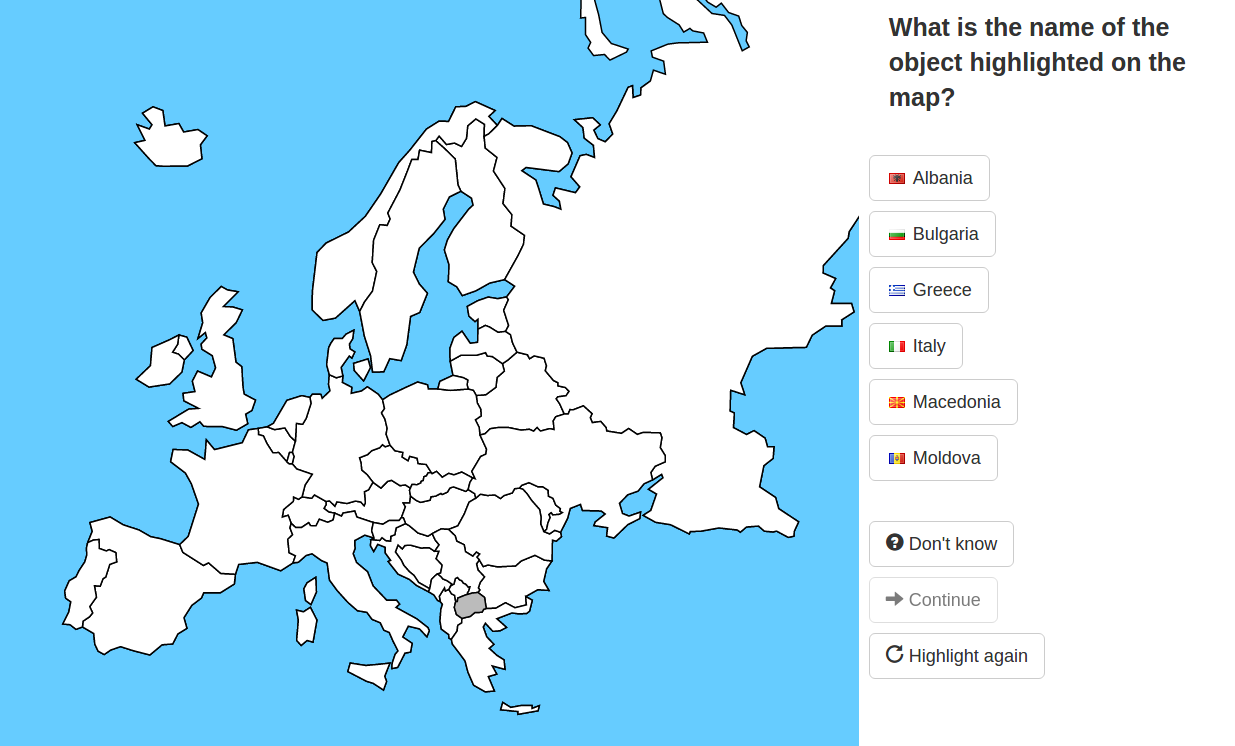
\includegraphics[width=\textwidth]{img/slepemapy}
  \caption{The screenshot corresponds to a multiple-choice question (with 5 distractors) requiring the student to identify the name of the highlighted country on an outline map of Europe.}
  \label{fig:slepemapy}
\end{figure}

The system provides an educational environment for learning of all kinds of geography facts, including world countries, cities, rivers, lakes, mountains, islands, Czech regions and many others. The system is also adaptive, i.e. it examines knowledge and skills of individual students adaptively based on previous answers by the selection of optimal repeat frequency, the type of question and its difficulty.

\section{Outline of the Thesis}

The first chapter covers the background for of thesis, we summarize the most relevant aspects of human memory and forgetting related to our research, we also describe characteristics of adaptive educational systems as well as mathematical models used in student modeling. In the second chapter, we propose models and their modifications that focus on timing information, we also describe the numerous methods and metrics used for parameter estimation. In the last chapter, we evaluate and compare the proposed models on several data sets containing different types of places (countries, mountains, rivers, etc.), we analyze the stability of models' predictions and perform further analysis.
